\documentclass{article}
\usepackage{graphicx} % Required for inserting images
\usepackage{hyperref}
\usepackage{booktabs}
\hypersetup{
    colorlinks=true,
    linkcolor=blue,
    urlcolor=blue
}


\title{Milestone for CV Final Project: NeRF}
\author{Xiaole Wang, Gaoxiang Ye (Equal Contribution)}
\date{January 17, 2024}

\begin{document}

\maketitle

\noindent
Additional results of our ablation studies (including images for each epoch and the PSNR curve), as well as our source code are at \href{https://disk.pku.edu.cn:443/link/98B88C53485C115705BB68F410388AD6}{this link}.

\section{Introduction}
Neural radiance fields (NeRFs) is a novel implicit 3D scene representation and a new approach to novel view synthesis, achieving outstanding visual fidelity. In this work, we attempt to implement one such NeRF and explore possible extensions to it, by generalize it to dynamic scenes and modifying it to target a non-NVS use case.

\section{Problem Statement}
\subsection{Description}
The problems we try to solve in this work are four-fold:
\begin{enumerate}
    \item Implement positional encoding and two-dimensional neural rendering: two important building blocks for NeRF.
    \item Implement a version of the original NeRF.
    \item Implement a neural radiance field that supports dynamic scenes. We plan to achieve this by adding time to the input of the neural network or by introducing an additional neural network that models the deformation field.
    \item Apply NeRF to a novel use case. The exact use case is still under research.
\end{enumerate}

\subsection{Dataset}

The following is the datasets we may use:

\href{https://drive.google.com/drive/folders/128yBriW1IG_3NJ5Rp7APSTZsJqdJdfc1}{Nerf-Data}

\href{https://www.tanksandtemples.org/}{Tanks and Temples -data}

We believe that the combination of these datasets comprehensively reflect NeRF's capacity to handle forward-facing and inward-facing, as well as synthetic and real-life scenes.

\subsection{Expected result}
Firstly, try to implement NeRF to fit one image and multi-view images. In this step, we will try our best to realize the achievements of predecessors. And realize NeRF for dynamic scenes step by step. Based on this, implement our own NeRF to make some innovation.

\subsection{Evaluation}
We plan to qualitatively assess the visual quality of the rendered results, as well as take into account metrics such as PSNR and SSIM.

\section{Technical Approach}
The ideas, algorithms and tricks used in the original NeRF and related works are well-conceived and have been thoroughly tested. Thus, we consider it best to draw inspiration from existing works as to our technical approach.

To be more specific, we will reference three prominent papers: \href{https://www.notion.so/Computer-Vision-Final-Project-207a8c05cf414d058a571843a250f990}{NeRF: Representing Scenes as Neural Radiance Fields for View Synthesis
} for vanilla NeRF, \href{https://arxiv.org/abs/2011.13961}{D-NeRF: Neural Radiance Fields for Dynamic Scenes} for deformation field-based dynamic NeRF, and \href{https://arxiv.org/abs/2011.12950}{Space-time Neural Irradiance Fields for Free-Viewpoint Video} for space-time neural network-based dynamic NeRF.

\section{Preliminary Results}
Now we have completed the task 1(Fit a single image with positional encoding), and examples for our preliminary result about task 1 are as following(The left is our result). We have also performed an ablation study on the effect of positional encoding, the number of frequencies in positional encoding, the width of the network, and its depth.

\begin{figure}[h]
    \centering
    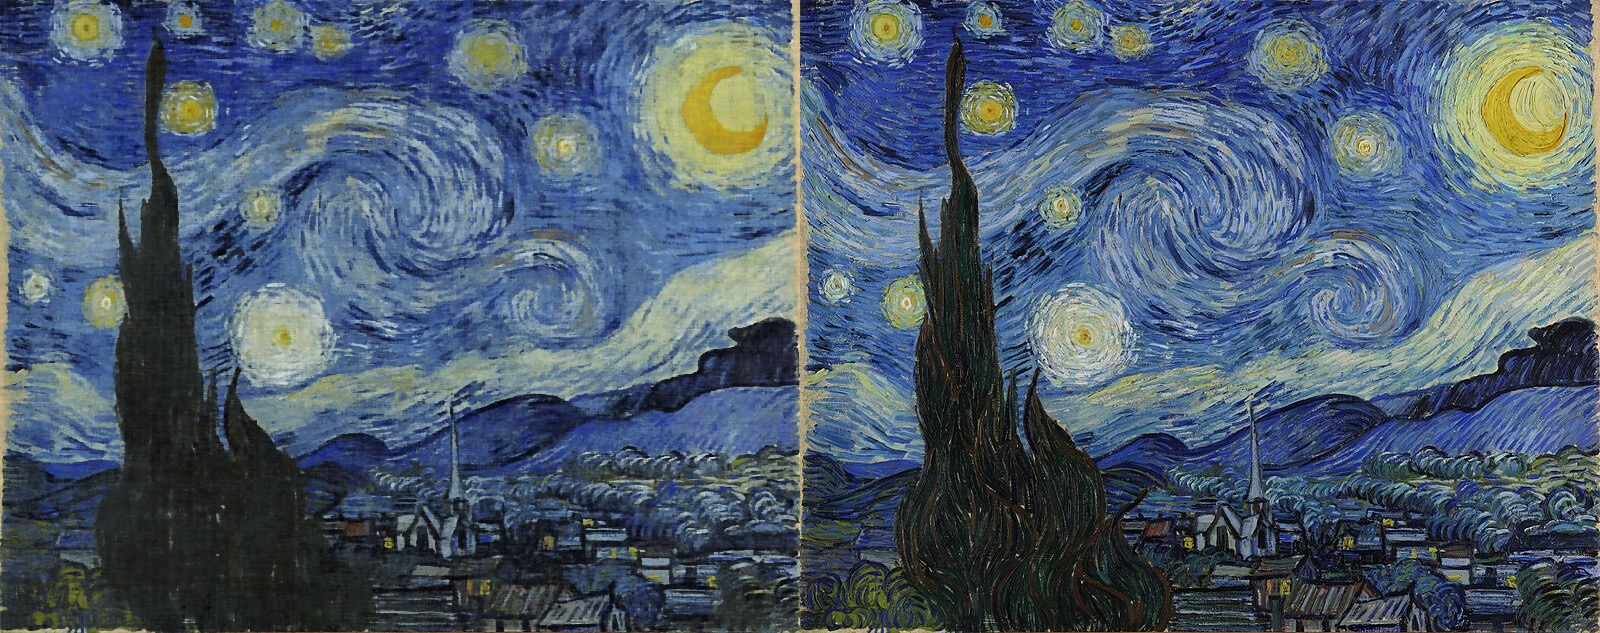
\includegraphics[width=0.6\textwidth]{starry_night.jpg}
    \caption{epoch=50, PSNR=23.37}
\end{figure}

\begin{figure}[h]
    \centering
    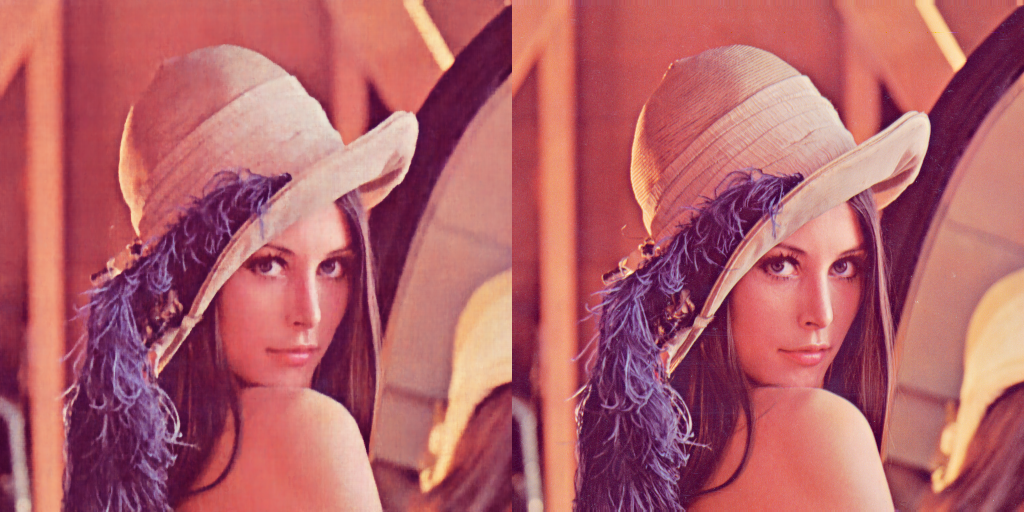
\includegraphics[width=0.6\textwidth]{lena.png}
    \caption{epoch=50, PSNR=31.08}
\end{figure}

\begin{figure}[h]
\subsection{Ablation Study on Positional Encoding}
    \begin{tabular}{c c}
       With positional encoding  & No positional encoding \\ 
       \midrule
        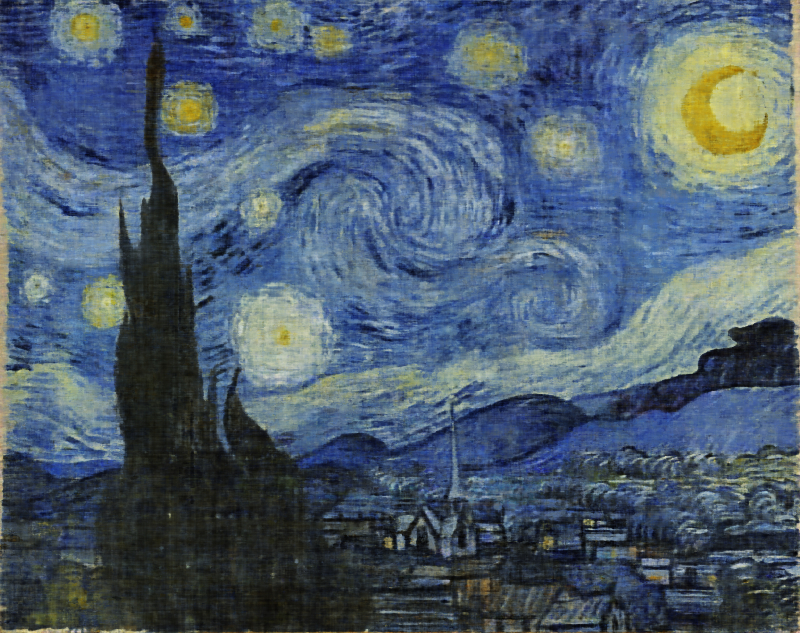
\includegraphics[width=0.5\linewidth]{no-15-norm-norm-pred.png} & 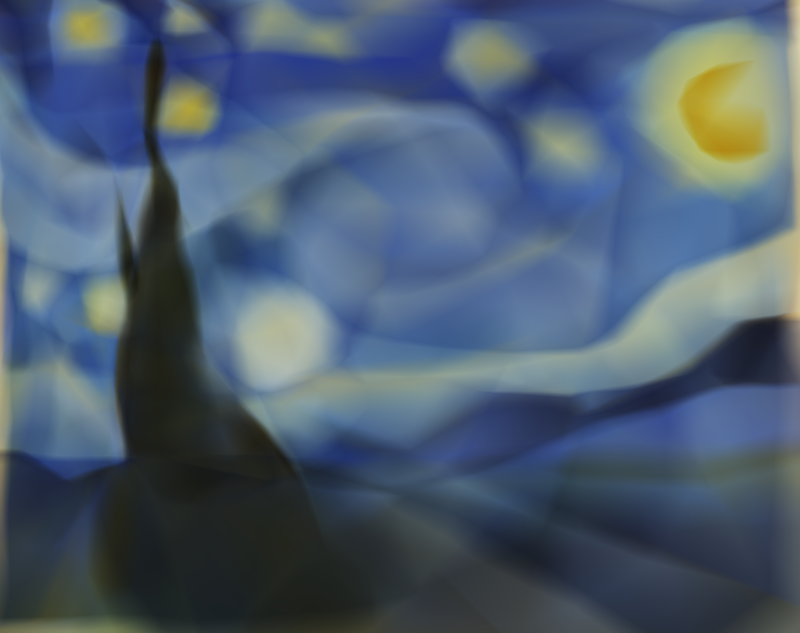
\includegraphics[width=0.5\linewidth]{pe-15-norm-norm-pred.png}
    \end{tabular}
    \caption{W/Wo Positional Encoding}

The difference between the results with and without positional encoding are apparent. The no-positional-encoding version struggles to capture fine details in the image, only rendering rough geometric shapes. We speculate this is due to the difference in neighboring pixel coordinates sufficiently emphasized in later elements in the positional encoding and the lack thereof in the no-positional-encoding version. Note the lack in representation power manifests as "blocky" artifacts.

\end{figure}

\begin{figure}[h]
\subsection{Ablation Study on Number of Frequencies in Positional Encoding}
    \begin{tabular}{c c c}
       L = 5  & L = 15 &  L = 30\\ 
       \midrule
        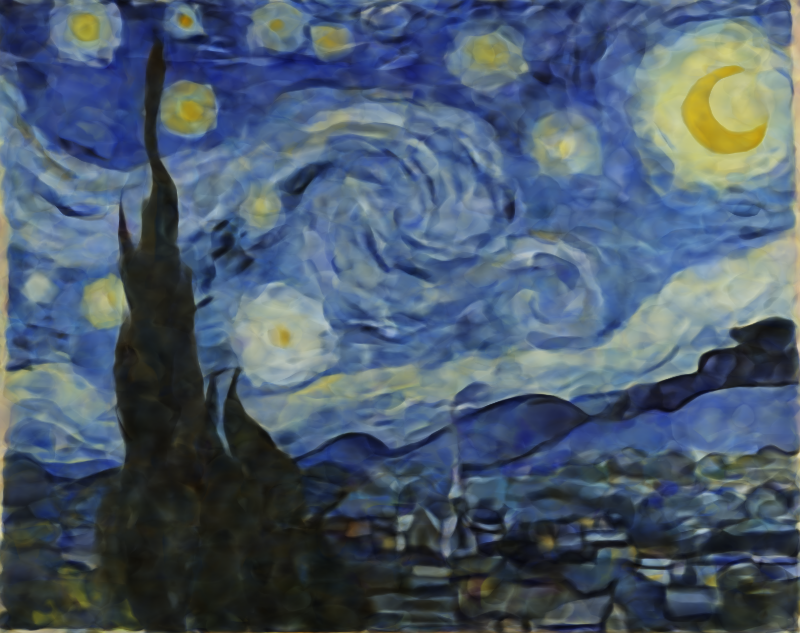
\includegraphics[width=0.3\linewidth]{pe-5-norm-norm-pred.png} & 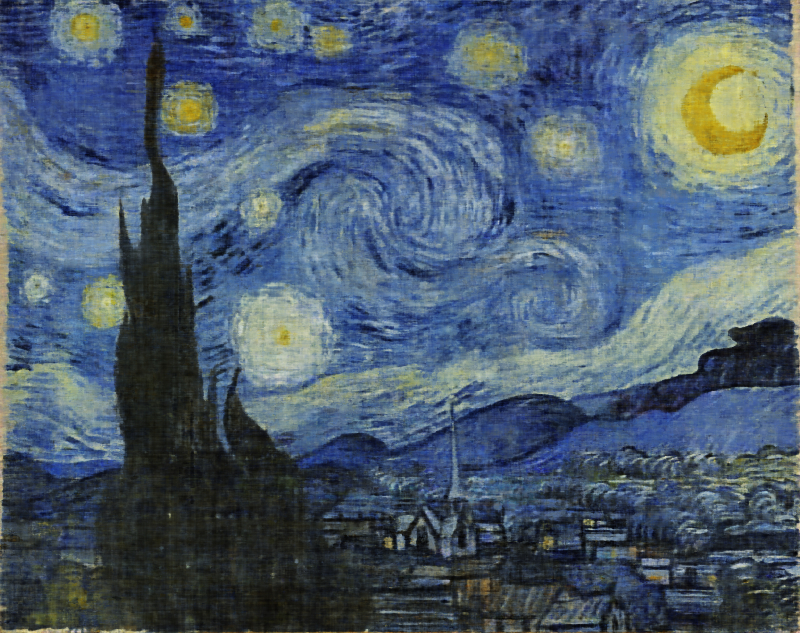
\includegraphics[width=0.3\linewidth]{no-15-norm-norm-pred.png} &
        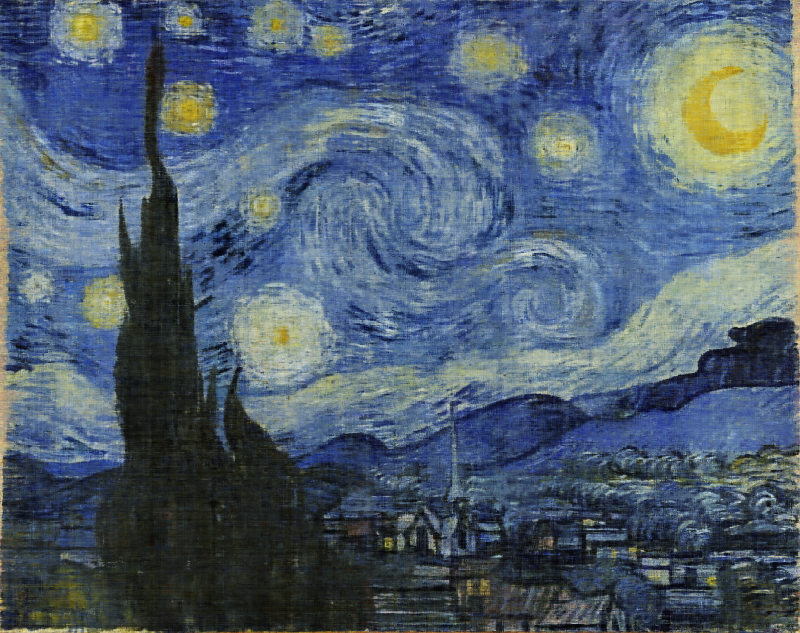
\includegraphics[width=0.3\linewidth]{pe-30-norm-norm-pred.png}
    \end{tabular}
    \caption{Diff frequencies in Positional Encoding}
    
Perhaps unsurprisingly, as the number of frequencies go up, so does the quality of the image. However, we also noted that the difference between L = 15 and L = 30 is not so apparent.
\end{figure}

\begin{figure}[h]
    \subsection{Ablation Study on Depth of Neural Network}
    \begin{tabular}{c c c}
       Shallow  & Baseline &  Deep\\ 
       \midrule
        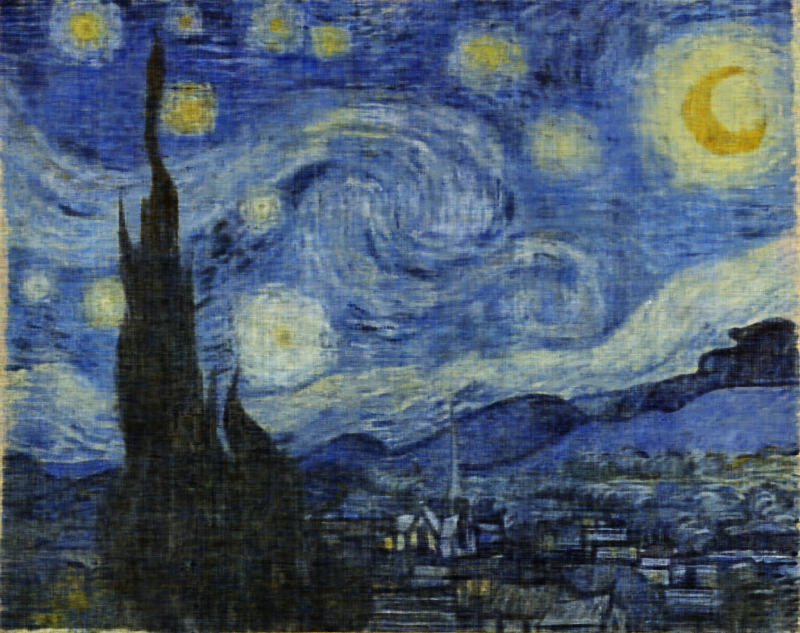
\includegraphics[width=0.3\linewidth]{pe-15-shallow-norm-pred.png} & 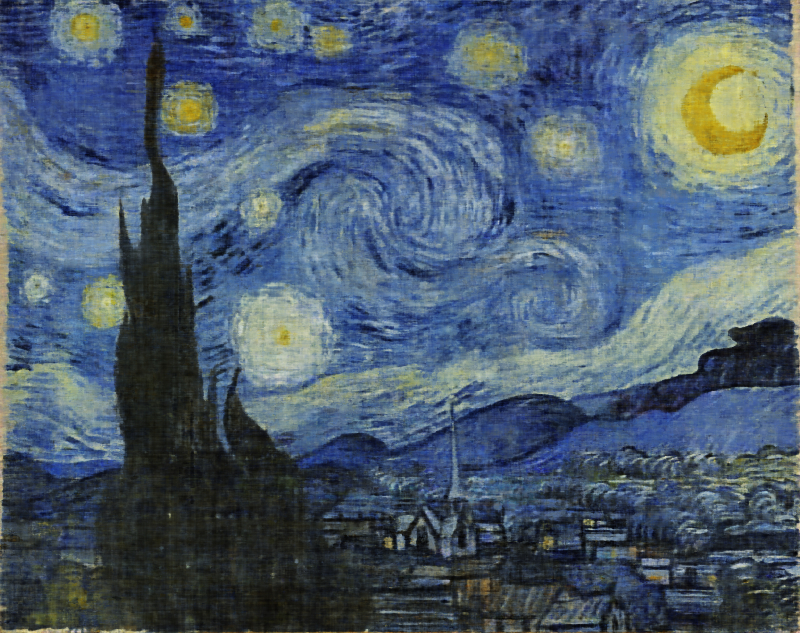
\includegraphics[width=0.3\linewidth]{no-15-norm-norm-pred.png} &
        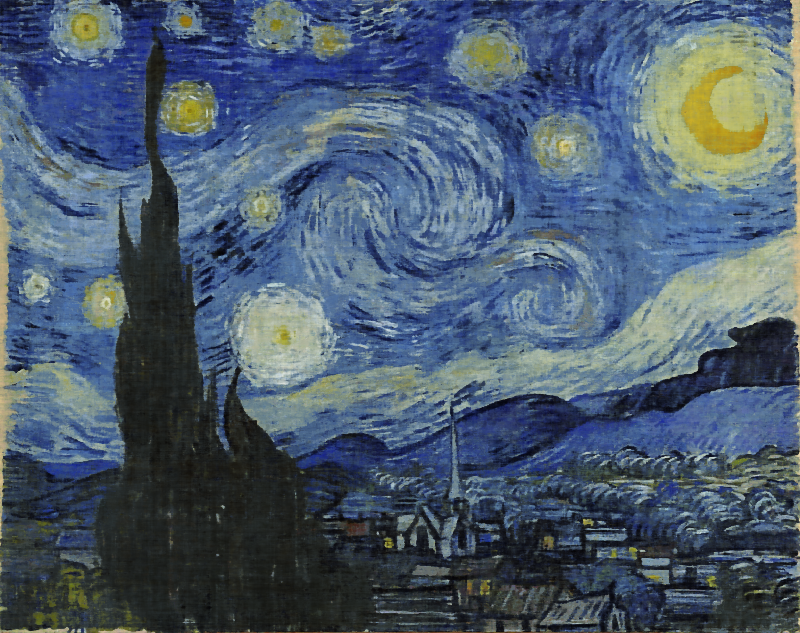
\includegraphics[width=0.3\linewidth]{pe-15-deep-norm-pred.png}
    \end{tabular}
    \caption{Diff depth of NN}
    
Much like with the number of frequencies, the visual quality goes up with the depth of the network, with diminishing returns.
\end{figure}

\begin{figure}[h]
    \subsection{Ablation Study on Width of Neural Network}
    \begin{tabular}{c c c}
       Thin  & Baseline &  Wide\\ 
       \midrule
    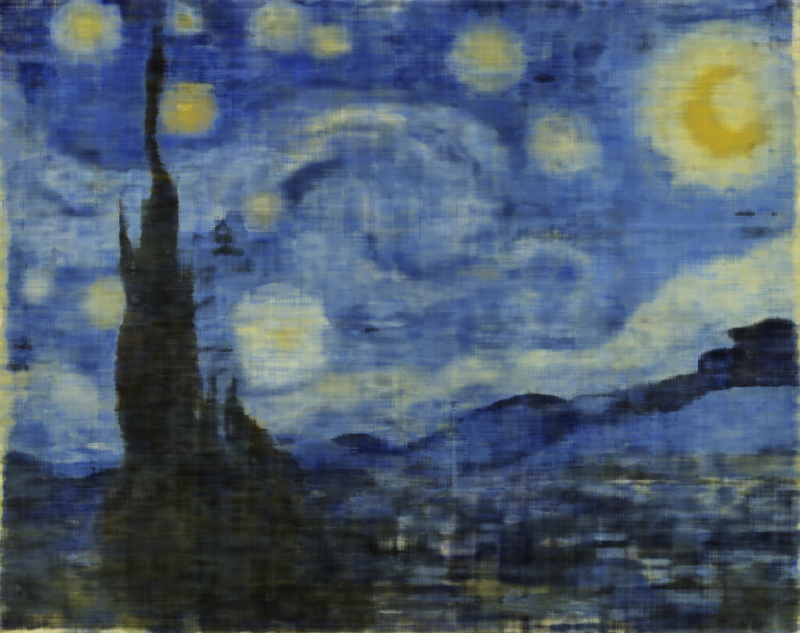
\includegraphics[width=0.3\linewidth]{pe-15-thin-norm-pred.png} & 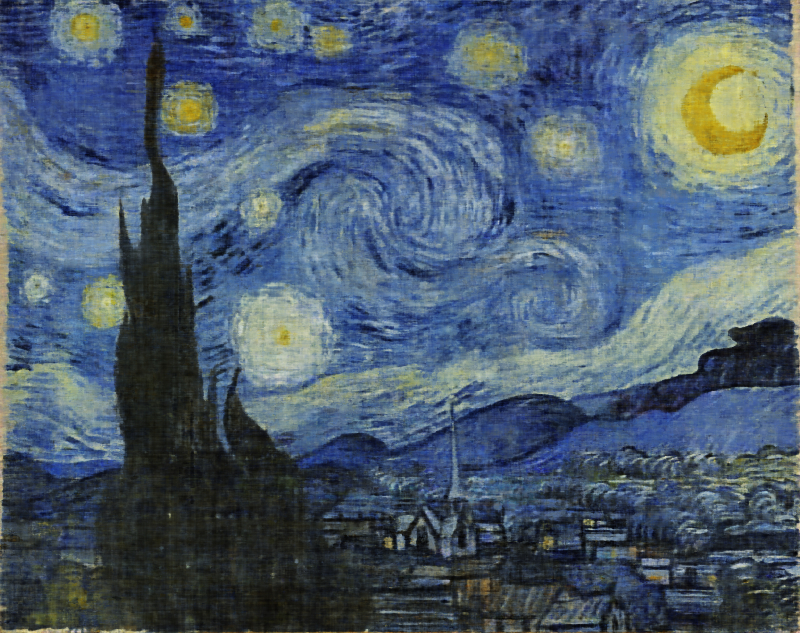
\includegraphics[width=0.3\linewidth]{no-15-norm-norm-pred.png} &
        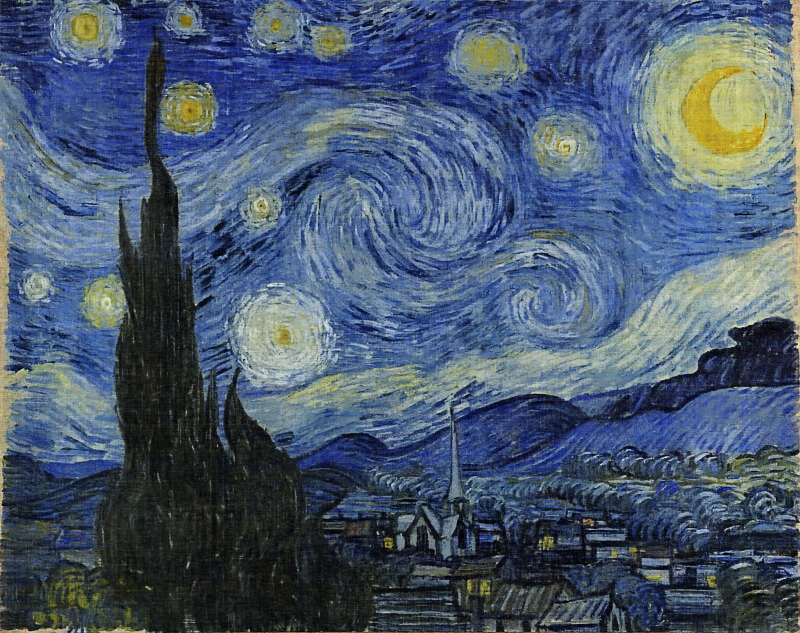
\includegraphics[width=0.3\linewidth]{pe-15-wide-norm-pred.png}
    \end{tabular}
    \caption{Diff width of NN}

Still, the visual quality goes up with the width of the network, also with diminishing returns. It seems that the width of the model has a larger impact than its depth. At the thinnest width, we can notice "gridy" artifacts.
\end{figure}

\end{document}
